\documentclass[../main.tex]{subfiles}

\begin{document}

    Für den Aufbau des Experimentes sind zwei Würfel mit den Dimensionen von 1.5m Seitenlänge und dem Gewicht von 2
    Kilogramm gegeben.
    Wie in der Abbildung~\ref{fig:2Lab_2dPictureNr1} zu entnehmen, ist linke Würfel Julia und der Rechte Romeo benannt.
    Daneben existiert eine Feder die horizontal an einer Wand befestigt ist.
    Bei dem gesammten Experimentes wird der Reibungswiederstand ignoriert.
    Ablauf des Experimentes:
 \begin{enumerate}
     \item Romeo wird mit einer konstanten Kraft (grüner Pfeil in Abbildung~\ref{fig:2Lab_2dPictureNr1}) auf
     2m/s nach rechts beschleunigt.
     \begin{figure}[H]
                 \begin{center}
                     \centerline{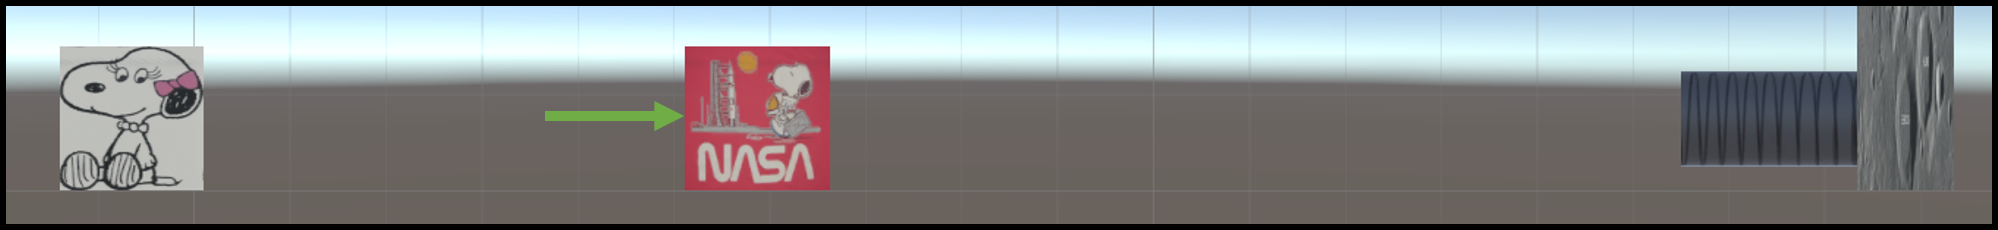
\includegraphics[width=155mm]{./images/2Lab_2dPictureNr1.png}}
                     \caption{Beschleunigung des Würfels}
                     \label{fig:2Lab_2dPictureNr1}
                 \end{center}
     \end{figure}
     \item Romeo trifft nun auf die Feder. Dabei soll die Federkonstante (gelber Pfeil in Abbildung~\ref{fig:2Lab_2dPictureNr2})
     so gewählt werden, dass Romeo elastisch zurückprallt ohne die Wand zu berühren.
     \begin{figure}[H]
               \begin{center}
                   \centerline{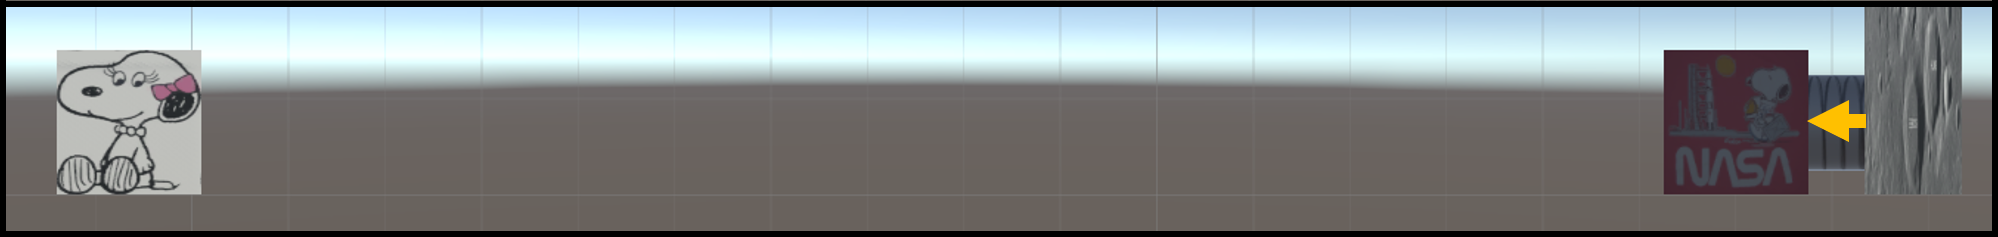
\includegraphics[width=155mm]{./images/2Lab_2dPictureNr2.png}}
                   \caption{Elastischer Zusammenstoss mit der Feder}
                   \label{fig:2Lab_2dPictureNr2}
               \end{center}
     \end{figure}
     \item Nach dem abgefederten Stoss gleitet Romeo zurück in die Richtung aus der er gekommen ist und stösst inelastisch mit Julia zusammen.
     Über einen FixedJoint haften die Beiden nun zusammen und gleiten mit der aufgeteilten Energie
     (blaue Pfeile in Abbildung~\ref{fig:2Lab_2dPictureNr3}) weiter nacht links.
     \begin{figure}[H]
                \begin{center}
                    \centerline{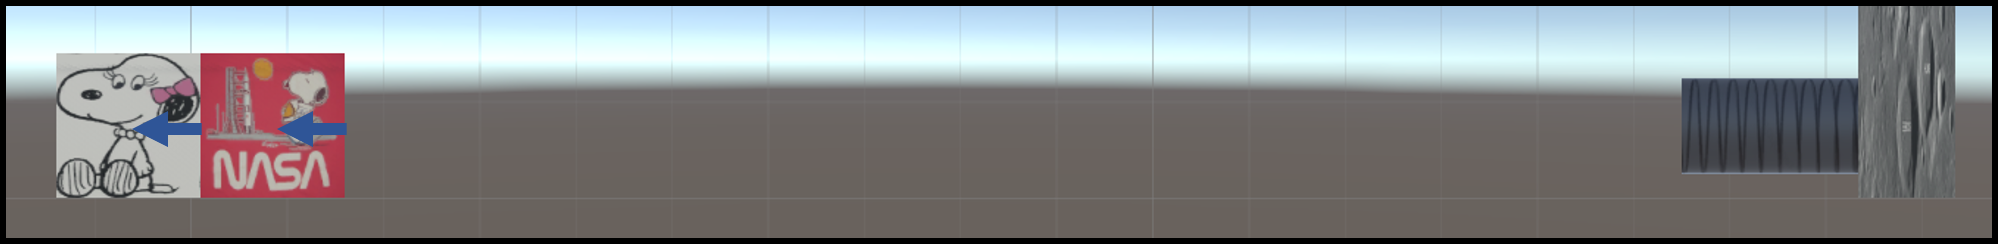
\includegraphics[width=155mm]{./images/2Lab_2dPictureNr3.png}}
                    \caption{Inelastischer zusammenstoss mit dem anderen Würfel}
                    \label{fig:2Lab_2dPictureNr3}
                \end{center}
     \end{figure}
 \end{enumerate}







\end{document}